\documentclass{beamer}

\usepackage{xltxtra}
\usepackage{graphicx}
%\usepackage[utf8]{inputenc}
\usepackage{fontspec}
\setmainfont{Verdana}
\setsansfont{Verdana}
\usepackage{tikz}
\usepackage{comment}
\usetikzlibrary{arrows,decorations.pathmorphing,backgrounds,fit,positioning,automata,calc,shapes.arrows,fadings}

\colorlet{mygray}{black!40}
\colorlet{mylightgray}{black!20}
\colorlet{mygreen}{green!60!black}
\definecolor{metroblue}{RGB}{0,59,126}
\definecolor{metroyellow}{RGB}{249,174,0}
\newcommand{\insertauthorpic}{
\includegraphics[width=1.446cm]{pics/philip.png}
\includegraphics[width=1.446cm]{pics/thomas.png}}
\newcommand{\footertext}{%
  \fontsize{5}{5}\selectfont\begin{minipage}{3mm}\vspace*{-1pt}\raggedleft\insertframenumber\end{minipage}\hspace*{3mm}
  © METRO AG.\hspace*{3mm}\insertshortauthor{}: \insertshorttitle{}
}
\newcommand{\datesize}{\fontsize{10}{10}\selectfont}
\newcommand{\metroslide}{%
{\setbeamercolor{background canvas}{bg=metroblue}
\begin{frame}[plain]
\centering

\includegraphics{pics/metro2.png}
\end{frame}
}
}



%TODO
\mode<presentation>
{
\setbeamerfont{block title}{size={}}
\usefonttheme{professionalfonts} % using non standard fonts for beamer
\usefonttheme{serif} % default family is serif
\setbeamercovered{transparent}
\setbeamertemplate{navigation bars}{}
\setbeamertemplate{navigation symbols}{}
\setbeamersize{text margin left=4mm}
\setbeamersize{text margin right=4mm}
\setbeamertemplate{itemize items}[ball]
\setbeamertemplate{enumerate items}[ball]
\setbeamertemplate{headline}{}
\setbeamertemplate{footline}{
  \begin{tikzpicture}[remember picture,overlay]
  \draw[metroblue] ($(current page.south west)+(0.6,0.6)$) -- ($(current page.south east)+(-3.5,0.6)$);
  \node (logosmall) at ($(current page.south east)+(-0.2,-0.1)$) [anchor=south east] {
\includegraphics[height=8mm]{metro.png}};
  \node[metroblue] (textline) at ($(current page.south west)+(0.8,0.13)$) [anchor=south west] {\footertext{}};
  \end{tikzpicture}
}
\defbeamertemplate*{title page}{metro}[1][]{
  \begin{tikzpicture}[remember picture,overlay]
  \node (logo) at (current page.north west) [anchor=north west] {
\includegraphics[height=\paperheight]{left.png}};
  \node[white] (title) at ($(logo)+(-0.7,0.65)$) [anchor=south west] {\fontsize{20}{20}\selectfont\textbf{\inserttitle}\par};
  \node[white] (subtitle) [below=0.7 of title.west,anchor=west] {\fontsize{12}{12}\selectfont\textbf{\insertsubtitle}\par};
  \node[white] (date) [below=0.9 of subtitle.west,anchor=west] {\datesize\insertdate,};
  \node[white] (place) [below=0.42 of date.west,anchor=west] {\datesize\selectfont\location};
  \node[white] (authorpic) [below=0.1 of place.south west,anchor=north west] {\insertauthorpic};
  \node[white] (author) [right=0.1 of authorpic.south east,anchor=south west] {\datesize\selectfont\insertauthor};
  \node[white] (textline) at ($(current page.south west)+(0.8,0.13)$) [anchor=south west] {\footertext{}};
  \end{tikzpicture}
}
\defbeamertemplate*{frametitle}{metro}[1][]{
  \vskip2mm%
  \hspace*{3mm}\fontsize{16}{12}\selectfont\textbf{\textcolor{metroblue}{\insertframetitle}}
}
}

% From: https://www.overleaf.com/latex/examples/listings-code-style-for-html5-css-html-javascript/htstpdbpnpmt#.WcjJM9_8vmE
% Stackexchange question: https://tex.stackexchange.com/questions/99500/listings-code-style-for-html5-css-html-javascript

\usepackage{color}
\definecolor{lightgray}{rgb}{0.95, 0.95, 0.95}
\definecolor{darkgray}{rgb}{0.4, 0.4, 0.4}
%\definecolor{purple}{rgb}{0.65, 0.12, 0.82}
\definecolor{editorGray}{rgb}{0.95, 0.95, 0.95}
\definecolor{editorOcher}{rgb}{1, 0.5, 0} % #FF7F00 -> rgb(239, 169, 0)
\definecolor{editorGreen}{rgb}{0, 0.5, 0} % #007C00 -> rgb(0, 124, 0)
\definecolor{orange}{rgb}{1,0.45,0.13}
\definecolor{olive}{rgb}{0.17,0.59,0.20}
\definecolor{brown}{rgb}{0.69,0.31,0.31}
\definecolor{purple}{rgb}{0.38,0.18,0.81}
\definecolor{lightblue}{rgb}{0.1,0.57,0.7}
\definecolor{lightred}{rgb}{1,0.4,0.5}
\usepackage{upquote}
\usepackage{listings}
% CSS
\lstdefinelanguage{CSS}{
  keywords={color,background-image:,margin,padding,font,weight,display,position,top,left,right,bottom,list,style,border,size,white,space,min,width, transition:, transform:, transition-property, transition-duration, transition-timing-function},
  sensitive=true,
  morecomment=[l]{//},
  morecomment=[s]{/*}{*/},
  morestring=[b]',
  morestring=[b]",
  alsoletter={:},
  alsodigit={-}
}

% JavaScript
\lstdefinelanguage{JavaScript}{
  morekeywords={typeof, new, true, false, catch, function, return, null, catch, switch, var, if, in, while, do, else, case, break},
  morecomment=[s]{/*}{*/},
  morecomment=[l]//,
  morestring=[b]",
  morestring=[b]'
}

\lstdefinelanguage{HTML5}{
  language=html,
  sensitive=true,
  alsoletter={<>=-},
  morecomment=[s]{<!-}{-->},
  tag=[s],
  otherkeywords={
  % General
  >,
  % Standard tags
    <!DOCTYPE,
  </html, <html, <head, <title, </title, <style, </style, <link, </head, <meta, />,
    % body
    </body, <body,
    % Divs
    </div, <div, </div>,
    % Paragraphs
    </p, <p, </p>,
    % scripts
    </script, <script,
  % More tags...
  <canvas, /canvas>, <svg, <rect, <animateTransform, </rect>, </svg>, <video, <source, <iframe, </iframe>, </video>, <image, </image>, <header, </header, <article, </article
  },
  ndkeywords={
  % General
  =,
  % HTML attributes
  charset=, src=, id=, width=, height=, style=, type=, rel=, href=,
  % SVG attributes
  fill=, attributeName=, begin=, dur=, from=, to=, poster=, controls=, x=, y=, repeatCount=, xlink:href=,
  % properties
  margin:, padding:, background-image:, border:, top:, left:, position:, width:, height:, margin-top:, margin-bottom:, font-size:, line-height:,
    % CSS3 properties
  transform:, -moz-transform:, -webkit-transform:,
  animation:, -webkit-animation:,
  transition:,  transition-duration:, transition-property:, transition-timing-function:,
  }
}

\lstdefinestyle{htmlcssjs} {%
  % General design
%  backgroundcolor=\color{editorGray},
  basicstyle={\footnotesize\ttfamily},
  frame=none,
  % line-numbers
  xleftmargin={0.75cm},
  numbers=left,
  stepnumber=1,
  firstnumber=1,
  numberfirstline=true,
  % Code design
  identifierstyle=\color{black},
  keywordstyle=\color{blue}\bfseries,
  ndkeywordstyle=\color{editorGreen}\bfseries,
  stringstyle=\color{editorOcher}\ttfamily,
  commentstyle=\color{brown}\ttfamily,
  % Code
  language=HTML5,
  alsolanguage=JavaScript,
  alsodigit={.:;},
  tabsize=2,
  showtabs=false,
  showspaces=false,
  showstringspaces=false,
  extendedchars=true,
  breaklines=true,
  % German umlauts
  literate=%
  {Ö}{{\"O}}1
  {Ä}{{\"A}}1
  {Ü}{{\"U}}1
  {ß}{{\ss}}1
  {ü}{{\"u}}1
  {ä}{{\"a}}1
  {ö}{{\"o}}1
}
%
\lstdefinestyle{py} {%
language=python,
literate=%
*{0}{{{\color{lightred}0}}}1
{1}{{{\color{lightred}1}}}1
{2}{{{\color{lightred}2}}}1
{3}{{{\color{lightred}3}}}1
{4}{{{\color{lightred}4}}}1
{5}{{{\color{lightred}5}}}1
{6}{{{\color{lightred}6}}}1
{7}{{{\color{lightred}7}}}1
{8}{{{\color{lightred}8}}}1
{9}{{{\color{lightred}9}}}1,
basicstyle=\footnotesize\ttfamily, % Standardschrift
numbers=left,               % Ort der Zeilennummern
%numberstyle=\tiny,          % Stil der Zeilennummern
%stepnumber=2,               % Abstand zwischen den Zeilennummern
numbersep=5pt,              % Abstand der Nummern zum Text
tabsize=4,                  % Groesse von Tabs
extendedchars=true,         %
breaklines=true,            % Zeilen werden Umgebrochen
keywordstyle=\color{blue}\bfseries,
frame=b,
commentstyle=\color{brown}\itshape,
stringstyle=\color{editorOcher}\ttfamily, % Farbe der String
showspaces=false,           % Leerzeichen anzeigen ?
showtabs=false,             % Tabs anzeigen ?
xleftmargin=17pt,
framexleftmargin=17pt,
framexrightmargin=5pt,
framexbottommargin=4pt,
%backgroundcolor=\color{lightgray},
showstringspaces=false,      % Leerzeichen in Strings anzeigen ?
}


\begin{document}

\title[React and Reflux]{REACT AND REFLUX:}
\subtitle{Components, Actions, Stores, and State}
\author[P.\ Baues, T.\ Str\"oder]{Philip Baues and Thomas Str\"oder}
\date{28./29.\ September 2017}
\newcommand{\location}{\texttt{code.talks} Hamburg}

\metroslide

{\setbeamercolor{background canvas}{bg=metroblue}
\begin{frame}[plain]
\titlepage
\end{frame}
}

\begin{comment}
Abstract:
React is currently one of the most popular ingredients of modern web applications. It is a component-based JavaScript library supporting the decomposition of big web applications into small parts, especially following principles like single responsibility and separation of concerns. However, on its own it lacks concise support for transversal state handling when parts of an application should alter the state of another part and these parts are not in a father-child-like relationship. To this end, the Reflux JavaScript library adds actions and stores for state handling.

In this talk, we will have a look at general patterns how to use React components together with Reflux stores and actions to build a responsive web application. Here, the focus is on state: When and where to (not) have it and how to deal with it using the facilities React and Reflux are offering. We illustrate these concepts with a small web shop example. In addition to that, we also address common mistakes and how to avoid them.
\end{comment}

\begin{frame}\frametitle{Drilled down webshop example}
\centering
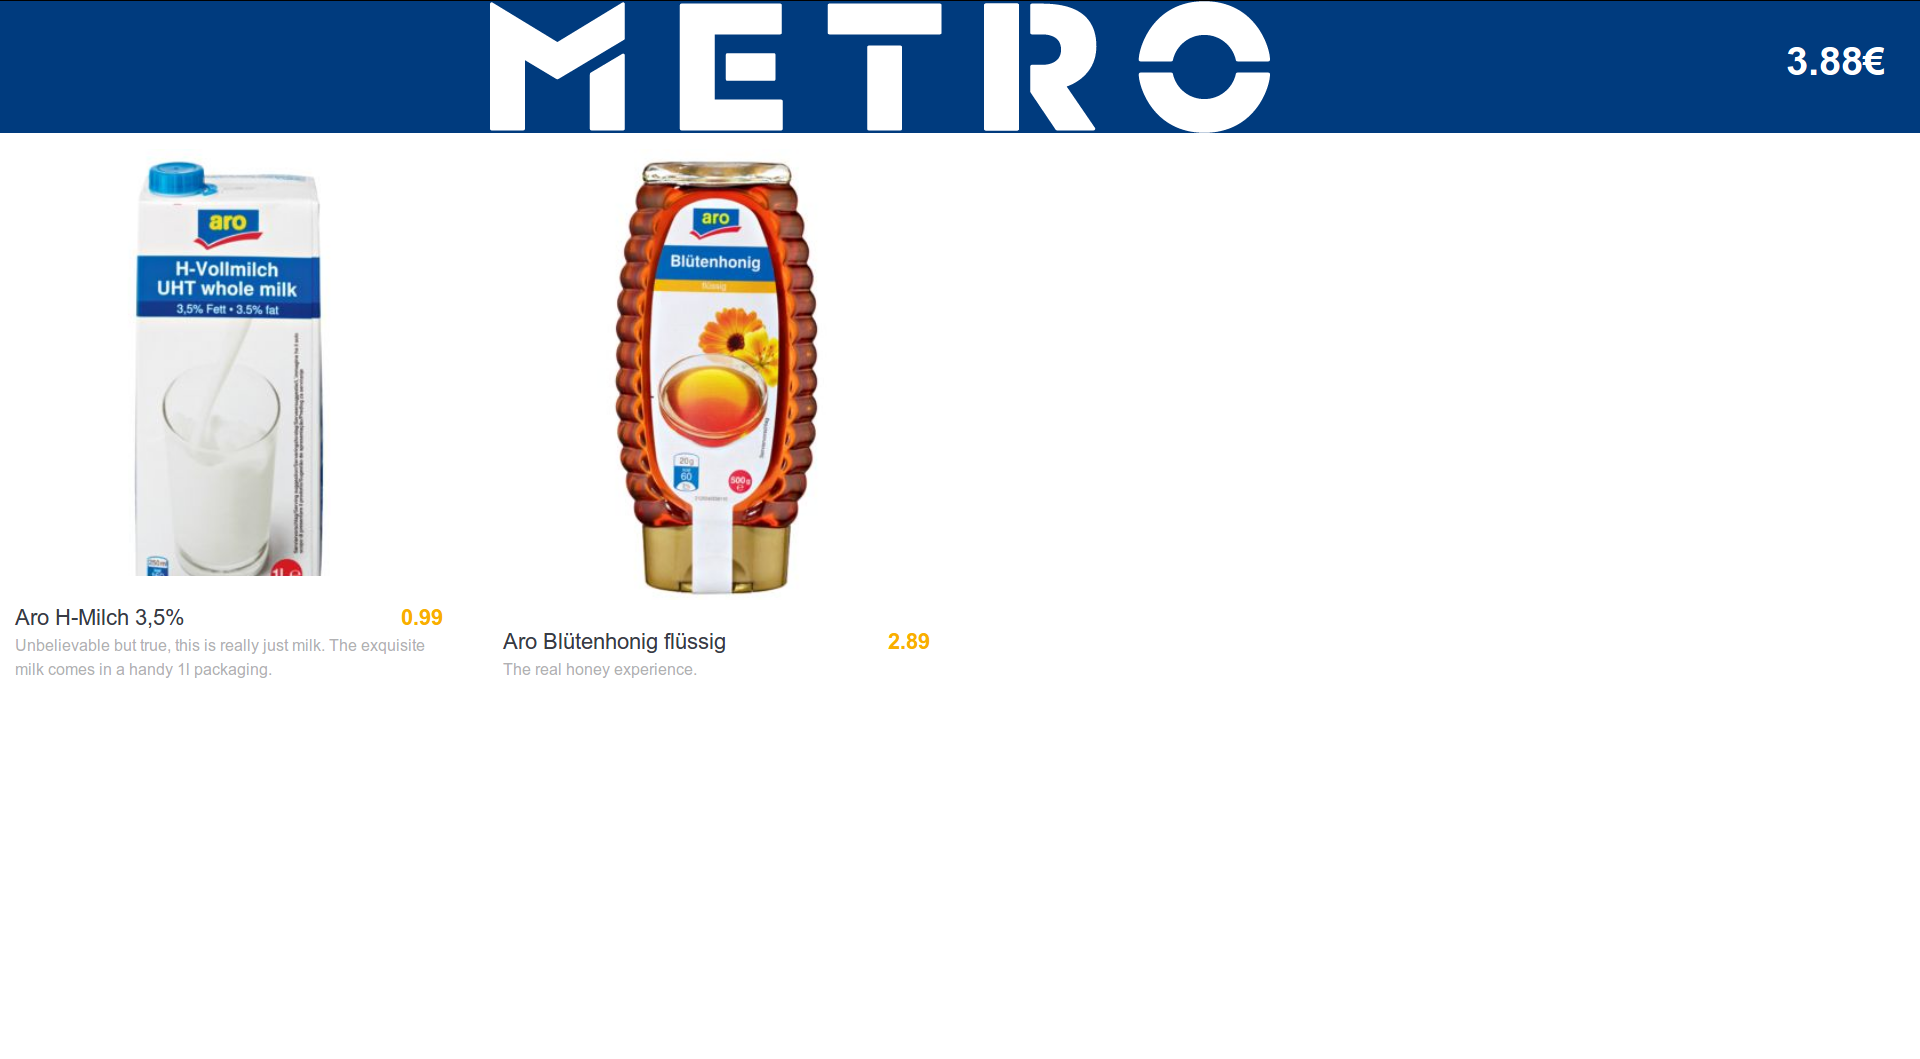
\includegraphics[width=.99\linewidth,height=.85\textheight,keepaspectratio]{pics/ExampleWebshop.png}
\end{frame}

\begin{frame}\frametitle{Why React?}
\centering
\begin{tikzpicture}
\visible<2->{\node[anchor=north west] (text1) at (0,6.1) {declarative view abstraction};}
\visible<3->{\fill[draw=metroblue,fill=metroblue!50,rounded corners=10] (6,0) rectangle (10,3);}
\visible<3->{\node[anchor=north west] at (6.1,2.9) {Component};}
\visible<4->{\fill[draw=metroyellow,fill=metroyellow!50,rounded corners=10] (6.9,0.1) rectangle (9.9,2.1);}
\visible<4->{\node[anchor=north west] at (7,2) {\small Component};}
\visible<6->{\fill[draw=metroblue,fill=metroblue!50,rounded corners=10] (6,3.1) rectangle (10,6.1);}
\visible<6->{\node[anchor=north west] at (6.1,6) {Component};}
\visible<5->{\node (text2) [below=of text1.west, anchor=west] {decoupling};}
\visible<7->{\node (text3) [below=of text2.west, anchor=west] {easy testing};}
\visible<8->{\node (text4) [below=of text3.west, anchor=west] {fast rendering};}
\end{tikzpicture}
\end{frame}

\begin{frame}\frametitle{React Components}
\centering
\tikzfading[name=fade left,
right color=transparent!0,
left color=transparent!100]
\begin{tikzpicture}
\node (component) {Component};
\visible<3->{\node (proparrow) [above left=0.1 of component,single arrow,shape border uses incircle,
shape border rotate=315,fill=metroblue,minimum height=2cm,path fading=fade left,fading transform={rotate=315}] {};}
\visible<3->{\node [above left=0.1 of proparrow] {\phantom{t}props};}
\visible<5->{\node (statearrow) [above right=0.1 of component,double arrow,shape border uses incircle,
shape border rotate=225,fill=red,minimum height=2cm] {};}
\visible<5->{\node [above right=0.1 of statearrow] {state\phantom{p}};}
\visible<2->{\node (renderarrow) [below=0.1 of component,single arrow,shape border uses incircle,
shape border rotate=270,fill=mygreen,minimum height=2cm,path fading=fade left,fading transform={rotate=270}] {};}
\visible<2->{\node [below=0.1 of renderarrow] {rendering};}
\visible<4->{\node (lifearrow) [above=0.1 of component,double arrow,shape border uses incircle,shape border rotate=90,
fill=red,minimum height=2cm] {};}
\visible<4->{\node [above=0.1 of lifearrow] {lifecycle};}
\end{tikzpicture}
\end{frame}

\begin{frame}[fragile]\frametitle{React Components \textendash{} Example}
\begin{lstlisting}[style=htmlcssjs]
class Article extends React.Component {

    render() {
        const article = this.props.article;
        return (
            <div key={article.id} className="col">
                <div className="article">
                    <img src={article.image}/>
                    <span>{article.name}</span>
                    <span>{article.price}</span>
                </div>
            </div>
        );
    }
}
\end{lstlisting}
\end{frame}

\begin{frame}\frametitle{Components}
\centering
\tikzfading[name=fade left,
right color=transparent!0,
left color=transparent!100]
\begin{tikzpicture}
\node (component) {Component};
\node (proparrow) [above left=0.1 of component,single arrow,shape border uses incircle,
shape border rotate=315,fill=metroblue,minimum height=2cm,path fading=fade left,fading transform={rotate=315}] {};
\node [above left=0.1 of proparrow] {\phantom{t}props};
\visible<3->{\node (statearrow) [above right=0.1 of component,single arrow,shape border uses incircle,
shape border rotate=225,fill=red,minimum height=2cm,path fading=fade left,fading transform={rotate=225}] {};}
\visible<-2>{\node (statearrow2) [above right=0.1 of component,double arrow,shape border uses incircle,
shape border rotate=225,fill=red,minimum height=2cm] {};}
\node [above right=0.1 of statearrow] {state\phantom{p}};
\node (renderarrow) [below=0.1 of component,single arrow,shape border uses incircle,
shape border rotate=270,fill=mygreen,minimum height=2cm,path fading=fade left,fading transform={rotate=270}] {};
\node [below=0.1 of renderarrow] {rendering};
\visible<-1>{\node (lifearrow) [above=0.1 of component,double arrow,shape border uses incircle,shape border rotate=90,
fill=red,minimum height=2cm] {};}
\visible<-1>{\node [above=0.1 of lifearrow] {lifecycle};}
\end{tikzpicture}
\end{frame}

\begin{frame}\frametitle{Why Reflux?}
\centering
\begin{tikzpicture}
\node[anchor=north west] (text1) at (0,6.1) {declarative view abstraction};
\fill[draw=metroblue,fill=metroblue!50,rounded corners=10] (6,0) rectangle (10,3);
\node[anchor=north west] at (6.1,2.9) {Component};
\fill[draw=metroyellow,fill=metroyellow!50,rounded corners=10] (6.9,0.1) rectangle (9.9,2.1);
\node[anchor=north west] at (7,2) {\small Component};
\fill[draw=metroblue,fill=metroblue!50,rounded corners=10] (6,3.1) rectangle (10,6.1);
\node[anchor=north west] at (6.1,6) {Component};
\visible<2->{\fill[draw=red,fill=red!50,rounded corners=10] (3.5,3.1) rectangle (5.5,5.1);}
\visible<2->{\node[anchor=north west] at (3.6,5) {Store};}
\node (text2) [below=of text1.west, anchor=west] {\alt<3->{\textcolor{red}{decoupling}}{decoupling}};
\node (text3) [below=of text2.west, anchor=west] {\alt<4->{\textcolor{red}{easy testing}}{easy testing}};
\node (text4) [below=of text3.west, anchor=west] {fast rendering};
\visible<5->{\node (text5) [below=of text4.west, anchor=west] {\textcolor{red}{transversal state handling}};}
\visible<2->{\draw (5.5,4.1) edge[<->,red,thick] (6,4.1);}
\visible<2->{\draw (5.4,3.2) edge[<->,red,thick] (6.1,2.9);}
\end{tikzpicture}
\end{frame}

\begin{frame}\frametitle{Data Flow}
\centering
\begin{tikzpicture}
[node/.style={rectangle,draw=black,thick,inner sep=5pt},
edge/.style={->,thick},
connect/.style={->,thick,dashed}]
\node[node] (action) {Action};
\node[node] (component) [below left=2 of action] {Component};
\node[node] (store) [below right=2 of action] {Store};
\visible<2->{\draw (component) edge[edge,in=180,out=90] node[auto] {calls} (action);}
\visible<3->{\draw (action) edge[edge,in=90,out=0] node[auto] {executes} (store);}
\visible<4->{\draw (store) edge[edge,in=270,out=270] node[auto] {sets state} (component);}
\visible<5->{\draw (component) edge[connect,bend right=30] node[auto,swap] {sets store(s)} (store);}
\visible<6->{\draw (store) edge[connect,in=270,out=180] node[auto] {listens to} (action);}
\end{tikzpicture}
\end{frame}

\begin{comment}
Notes on Reflux components:
* Set multiple stores by setting this.stores (the plural) and setting it to an Array of store classes.
* Set a this.storeKeys Array to restrict only certain parts of the store being mixed into the component state.
\end{comment}
\begin{frame}\frametitle{Reflux Components}
\centering
\tikzfading[name=fade left,
right color=transparent!0,
left color=transparent!100]
\begin{tikzpicture}
\node (component) {Component};
\node (proparrow) [above left=0.1 of component,single arrow,shape border uses incircle,
shape border rotate=315,fill=metroblue,minimum height=2cm,path fading=fade left,fading transform={rotate=315}] {};
\node [above left=0.1 of proparrow] {\phantom{t}props};
\node (statearrow) [above right=0.1 of component,single arrow,shape border uses incircle,
shape border rotate=225,fill=red,minimum height=2cm,path fading=fade left,fading transform={rotate=225}] {};
\node [above right=0.1 of statearrow] {state\phantom{p}};
\node (renderarrow) [below=0.1 of component,single arrow,shape border uses incircle,
shape border rotate=270,fill=mygreen,minimum height=2cm,path fading=fade left,fading transform={rotate=270}] {};
\node [below=0.1 of renderarrow] {rendering};
\visible<3->{\node (setarrow) [right=0.1 of component,single arrow,fill=red,minimum height=2cm,path fading=fade left] {};}
\visible<3->{\node [right=0.1 of setarrow] {setStore(s)};}
\visible<2->{\node [above=2.5 of component] {extend React components};}
\visible<4->{\node [below left=0.5 of component] {\begin{minipage}{3cm}\begin{center}only\\interaction\\logic\end{center}\end{minipage}};}
\visible<5->{\node [below right=0.5 of component] {\begin{minipage}{3cm}\begin{center}treat state as\\read-only\end{center}\end{minipage}};}
\end{tikzpicture}
\end{frame}

\begin{frame}\frametitle{Actions}
\centering
\begin{tikzpicture}
\node (action) {Action};
\visible<2->{\node [above=of action] {just a function};}
\visible<3->{\node (callarrow) [below left=0.1 of action,single arrow,shape border uses incircle,
shape border rotate=45,fill=metroblue,minimum height=2cm,path fading=fade left,fading transform={rotate=45}] {};}
\visible<3->{\node [below left=0.1 of callarrow] {\begin{minipage}{3cm}\begin{center}called by component\end{center}\end{minipage}};}
\visible<4->{\node (transarrow) [below right=0.1 of action,single arrow,shape border uses incircle,
shape border rotate=315,fill=mygreen,minimum height=2cm,path fading=fade left,fading transform={rotate=315}] {};}
\visible<4->{\node [below right=0.1 of transarrow] {\begin{minipage}{3cm}\begin{center}transports payload\end{center}\end{minipage}};}
\end{tikzpicture}
\end{frame}

\begin{frame}\frametitle{Stores}
\centering
\begin{tikzpicture}
\node (store) {Store};
\visible<2->{\node [above=of store] {state handler};}
\visible<3->{\node (listenarrow) [below left=0.1 of store,single arrow,shape border uses incircle,
shape border rotate=45,fill=metroblue,minimum height=2cm,path fading=fade left,fading transform={rotate=45}] {};}
\visible<3->{\node [below left=0.1 of listenarrow] {\begin{minipage}{3cm}\begin{center}listens to actions\end{center}\end{minipage}};}
\visible<4->{\node (setarrow) [below right=0.1 of store,single arrow,shape border uses incircle,
shape border rotate=315,fill=mygreen,minimum height=2cm,path fading=fade left,fading transform={rotate=315}] {};}
\visible<4->{\node [below right=0.1 of setarrow] {\begin{minipage}{3cm}\begin{center}sets state of components\end{center}\end{minipage}};}
\visible<5->{\node [left=of store] {\begin{minipage}{3cm}\begin{center}stores\\actual state\end{center}\end{minipage}};}
\visible<6->{\node [right=of store] {\begin{minipage}{3cm}\begin{center}only\\``data logic''\end{center}\end{minipage}};}
\end{tikzpicture}
\end{frame}

\begin{frame}[fragile]\frametitle{Reflux Components, Actions, and Stores \textendash{} Example}
\begin{lstlisting}[style=htmlcssjs]
const Actions = Reflux.createActions([
    "loadArticles",
    "addToBasket",
    "removeFromBasket",
    "clearBasket"
]);
\end{lstlisting}
\end{frame}

\begin{frame}[fragile]\frametitle{Reflux Components, Actions, and Stores \textendash{} Example}
%\begin{frame}[fragile]\frametitle{Stores example}
\begin{lstlisting}[style=htmlcssjs]
class ArticleStore extends Reflux.Store {
    constructor() {
        super();
        this.state = {articles: []};
        this.listenTo(Actions.loadArticles, this.loadArticles);
    }
    loadArticles() {
          ArticleClient.loadArticles()
            .then(this.loadCompleted.bind(this))
            .catch(this.loadFailed.bind(this));
    }
    loadCompleted(newArticles) {
        this.setState({articles: newArticles});
    }
    loadFailed(response) {
        console.warn("Loading articles failed:", response);
    }
\end{lstlisting}
\end{frame}

\begin{comment}
Instead of loading the first bunch of articles in componentDidMount or componentWillMount one could do the following in the store:
Reflux.createStore({
    init: function() {
        this.state = "Init state";
    }
    getInitialState: function() {
        this.loadArticles();
    }
}
\end{comment}
\begin{frame}[fragile]\frametitle{Reflux Components, Actions, and Stores \textendash{} Example}
\begin{lstlisting}[style=htmlcssjs]
class ExampleWebshop extends Reflux.Component {
    constructor(props) {
        super(props);
        this.store = ArticleStore;
    }
    componentDidMount() {
        Actions.loadArticles();
    }
    render() {
        return (
            <div>
                <div className="row">
                    {this.state.articles.map(article =>
                        <Article article={article} />)}
                </div>
            </div>);
    }
}
\end{lstlisting}
\end{frame}

\begin{frame}\frametitle{Problematic state handling}
\begin{itemize}
\item Getter in stores
\item Unnecessary state in components
\item State vs. props
\end{itemize}
\end{frame}

\begin{frame}[fragile]\frametitle{Getter in stores \textendash{} Example}
\begin{lstlisting}[style=htmlcssjs]
const BasketStore =  Reflux.createStore({
    constructor() {
        this.basket = [];
        this.listenTo(Actions.addToBasket, this.addToBasket);
    },

    getBasket() {
        return this.basket;
    },

    addToBasket(article) {
        if (!this.isArticleInBasket(article)) {
            this.basket = this.basket.concat([article])
        }
        this.trigger(this.basket());
    }
};
\end{lstlisting}
\end{frame}

\begin{frame}[fragile]\frametitle{Getter in stores \textendash{} Example}
\begin{lstlisting}[style=htmlcssjs]
class Article extends Reflux.Component {
    render() {
        const article = this.props.article;
        return (
            <div className="article" >
                <img src={article.image}/>
                <span>{article.name}<span/>
                <span>{article.name}<span/>
                <div onClick={() => {
                    BasketStore.getBasket().indexOf(article.id) < 0
                    ? "Add to basket"
                    : "Remove from basket"}
                </div>
            </div>
        );
    }
}
\end{lstlisting}
\end{frame}

\begin{frame}[fragile]\frametitle{Unnecessary state in components \textendash{} Example}
\begin{lstlisting}[style=htmlcssjs]
class Article extends Reflux.Component {
    constructor(props) {
        super(props);
        this.store = BasketStore;
    }
    render() {
        return (
            <div className="article" onClick={() => {
                this.state.basket.indexOf(this.props.article) < 0
                ? "Add to basket"
                : "Remove from basket"}
            </div>
        );
    }
}
\end{lstlisting}
\end{frame}

\begin{frame}[fragile]\frametitle{State vs. props \textendash{} Example}
\begin{lstlisting}[style=htmlcssjs]
class Article extends Reflux.Component {
    constructor(props) {
        super(props);
    }
    render() {
        return (
            <div className="article" onClick={() => {
                this.props.articleIsAlreadyInBasket
                ? "Add to basket"
                : "Remove from basket"}
            </div>
        );
    }
}
\end{lstlisting}
\end{frame}

\begin{frame}\frametitle{How to handle state}
\vspace*{\fill}
\begin{center}
\begin{minipage}{.6\textwidth}
DON'T!
\end{minipage}
\end{center}
\vfill % equivalent to \vspace{\fill}
\end{frame}

\begin{frame}\frametitle{How to handle state\newline(if you have to)}
\begin{itemize}
\item Access state from as few components as possible
\item Do not alter state in a component directly
\item Extract state on a high level and hand it to child components via props
\item Stateless components
\end{itemize}
\end{frame}

\begin{frame}[fragile]\frametitle{Stateless component \textendash{} Example}
\begin{lstlisting}[style=htmlcssjs]
const ExampleWebshopHeader = ({sumPrice}) => {
    return (
        <div className="row webshop-header">
            <img className="logo" src="https://www.internet.com" />
            <div className="basket" 
                    onClick={() => Actions.clearBasket()}>
                <span>{sumPrice + "€"}</span>
            </div>
        </div>
    );
};

ExampleWebshopHeader.propTypes = {
    sumPrice: PropTypes.number.isRequired
};

export default ExampleWebshopHeader;
\end{lstlisting}
\end{frame}

\begin{frame}\frametitle{React and Reflux @METRO}
\centering
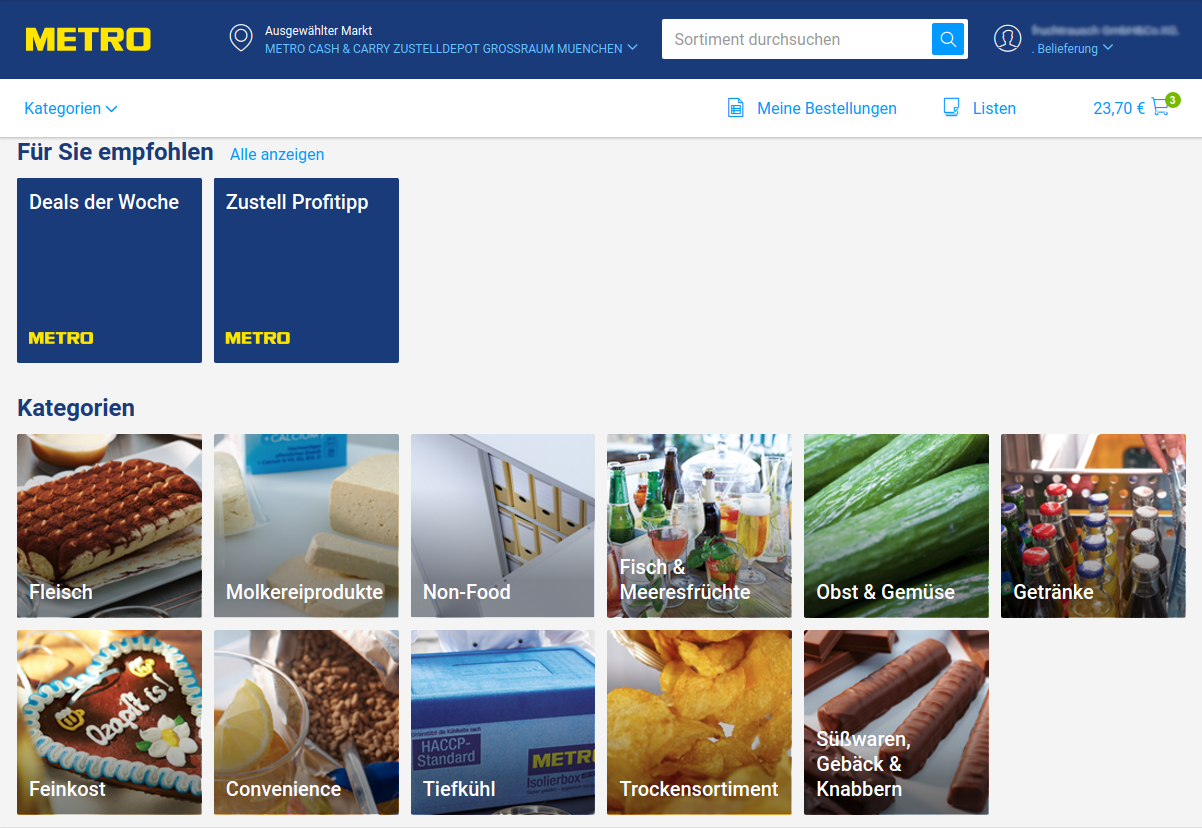
\includegraphics[width=.85\linewidth,height=.85\textheight,keepaspectratio]{pics/betty.png}
\end{frame}

\begin{frame}\frametitle{Tech Stack @METRO}
\centering
\begin{tikzpicture}
\visible<7->{\node at (8.5,6) {
\includegraphics[height=1cm]{pics/react.png}};}
\visible<6->{\node at (0,4) {
\includegraphics[height=1.5cm]{pics/cassandra.png}};}
\visible<2->{\node at (0,2) {\Large Docker};}
\visible<5->{\node at (3.5,0) {
\includegraphics[height=2cm]{pics/kubernetes.png}};}
\visible<8->{\node at (7,4.5) {\Large Java 8};}
\visible<12->{\node at (8,3) {
\includegraphics[height=1.5cm]{pics/haskell.jpg}};}
\visible<10->{\node at (9,4.5) {
\includegraphics[height=2cm]{pics/go.png}};}
\visible<11->{\node at (8,2) {\Large Clojure};}
\visible<13->{\node at (7.5,0) {
\includegraphics[height=1cm]{pics/latex.png}};}
\visible<9->{\node at (8.5,1) {
\includegraphics[height=1cm]{pics/scala.png}};}
\visible<2->{\node at (2.2,1.7) {
\includegraphics[height=1.3cm]{pics/container.png}};}
\visible<2->{\node at (3.5,1.7) {
\includegraphics[height=1.3cm]{pics/container.png}};}
\visible<2->{\node at (4.8,1.7) {
\includegraphics[height=1.3cm]{pics/container.png}};}
\visible<3->{\node at (3.5,3) {\Large \textbf{REST API}};}
\visible<4->{\node at (3.5,6) {\url{http://domain/service/endpoint}};}
\visible<4->{\node at (3.5,4.5) [single arrow,shape border uses incircle,
shape border rotate=270,fill=metroblue,minimum height=2cm,path fading=fade left,fading transform={rotate=270}] {};}
\end{tikzpicture}
\end{frame}

\end{document}
